% !TEX TS-program = pdflatex
% !TEX encoding = UTF-8 Unicode

\documentclass[11pt]{article} % use larger type; default would be 10pt

\usepackage[utf8]{inputenc} % set input encoding (not needed with XeLaTeX)
%%% PAGE DIMENSIONS
\usepackage{geometry} % to change the page dimensions
\geometry{a4paper} % or letterpaper (US) or a5paper or....
\usepackage{graphicx} % support the \includegraphics command and options

% \usepackage[parfill]{parskip} % Activate to begin paragraphs with an empty line rather than an indent


\title{Stay Frosty}
\author{Tigar Cyr and Matt Harrington}
%\date{} % Activate to display a given date or no date (if empty),
         % otherwise the current date is printed 

\begin{document}
\maketitle

\section{Introduction}

\subsection{Goal}

Our goal with Stay Frosty is to create a fun 2D platforming game exploring mechanics stemming from light.  We wanted to give the player an intimate relationship with light: a reason to be drawn to it, and at the same time to be made vulnerable by it.  We suspected that with shadows, reflections, refractions and manipulations of light sources, this core mechanic could serve as a platform for a variety of puzzles and experiences.  Our intended audience would be general public, for our game is a simple platformer and accessible to all age groups. \par

\subsection{Previous Work}
The biggest unknown and at the same time core of our project at the outset was the lighting engine.  For this project we would need a lighting simulation that would indicate to the player where exactly light reaches, and runs quickly enough to be incorporated into an interactive experience.  We both had experience with 3D raycasting from a previous assignment, but did not know how to take advantage of a reduction to 2D to increase performance.  We searched online for approaches and algorithms for handling lighting and by chance came across a project by Ewen Wang and Kevin Li, written in Processing, our language of choice, that solved many of the problems we had.  It simulates shadows in a 2D scene by intersecting rays of light with each polygon in the scene and drawing a polygon in the color of the light using these intersections as vertices.  Thier source code was freely available, albeit crudely written, so we began our project by studying and refactoring this code base so that we could extend it.  The original source we started from was about 200 lines of code written in Processing, and now our extension is roughly 1000.

\subsection{Approach}

We chose to make our game as a sketch within the Processing framework/language.  We chose this because of its similarity to Java, speed, portability, and wealth of built-in functions for rendering and geometry.  It should work well testing on most any laptop or desktop, running with decent framerate.  The drawback, though to choosing a sketch is that it is not as easily shared over the web, particularly to mobile devices.  However, we would not expect much difficulty converting the project to p5.js were we to pursue that route.\par

For our mechanics, we chose the following context/mechanic: Frosty is a snowman trying to get... somewhere.  As a snowman, he rolls around pretty slowly.  However, when he's in direct light, he warms up and melts, letting him slide around at higher speeds.  But this comes with the side effect of Frosty shrinking, and if he gets too small he simply melts away.  Luckily though, it's snowing outside, so if he shrinks and gets back into the shade, he'll slowly regrow to his original size.

\section{Methodology}

To extend the lighting simulation into a full-fledged game, we had some new features to implement:

\begin{enumerate}
	\item Collision Detection
	\item Motion and Controls
	\item Lighting Customizations
	\item Level Design
\end{enumerate}


\subsection{Collision Detection}

In order to implement any sort of game physics, we needed to implement basic collision detection for 2D polygons.  We have considered two main approaches to handle this robustly and efficiently.  First, basic particle physics: we could treat each vertex of each polygon as a separate particle and track collisions with other vertices and edges.  Second, we could check at each time step for collisions among polygons using the Separating Axis Theorem for convex polygons.  This approach is customized to polygons and fast, but restricts us to convex shapes and is not designed to incorporate motion.  For sake of efficiency, we have implemented Stay Frosty with the Separating Axis Theorem approach, checking intersections with the convex hull of a polygon's starting and ending location at each time step to account for motion.  This has kept our performance up, but comes with the drawback of a speed limit for the collision detection to work.  In future versions, we would like to further explore options based on particle physics.

\subsection{Motion and Controls}

While we were entirely fixed on the control scheme of moving left and right and jumping, there were numerous tweaks withing those controls to consider.  First, we had to decide how to handle the speed boost when entering light: we could either increase their speed as they enter the light, or increase it linearly, the longer they've been lit.  In order to give the player a prolonged sense of improvement, we decided on the latter, and to avoid winding up for high speeds, we reset a player's speed when they turn.  This choice, however caused issues with our collision detection when the player reached high speeds, so we put a cap on the speed.  
\par The other area where we had design choices to make was the jump.  Considering different possibilities, we decided to let the player lean and change their momentum slightly while in the air, but still stop them from really picking up speed in the air.  We see this as striking a balance between ease of use for players to land jumps with precision and realism.  After seeing the positive results, from this implementation, we are considering implementing a double-jump in future versions.

\subsection{Lighting Customizations}

In order to keep tracking of whether Frosty is in the light, we extended and replaced many of the data structures used in the lighting engine, so that we could track which intersections came from which shapes.  This allowed us to set a flag on each shape indicating whether or not it is lit.  We then took advantage of our understanding of the lighting algorithm to enable transparent objects, which are visible but do not interact with the light.  One final feature we have begun to plan, but do not yet have an implementation for is reflections; the lighting engine is not set up to handle reflections, but we have some ideas on how to hack it together: one such idea is to recast rays from reflective surfaces similarly to how the engine does it, but as if they were from a new light source.

\subsection{Level Design}

When it came to designing levels, we prioritized creating many unique and challenging layouts and courses instead of making the sprites and designs themselves pretty or detailed. We also wanted to introduce mechanics gradually and lightly. Therefore, the levels are sequenced in such a way that a player learrns first of the effects that light has on their movement and size, then of their ability to jump and plamtform. The levels in general are meant to increase in difficulty. We've had 7 people test the game so far. With next to no instruction, they all managed to pick up the mechanics right away. While they had difficulty finishing some of the levels, they never rage quit or yelled at us for having an unplayable game. Altogether, their feedback was constructive and positive.

\section{Results}

We judged the results of our project based on the performance, bugginess. and reception of our game.  In terms of performance, we are pleased with the fact that Stay Frosty has managed to maintain a framerate of 60fps on every machine we have tested on.  As for polish, we have designed our levels to hide the bugs in our collision detection system until they are resolved.  For example, while we still have a speed limit, players need never approach this speed to complete any of the levels.  Finally, the reception of our game, tested with roommates, classmates, and other friends, has been generally positive.  People tend to be impressed with the lighting particularly (which we cannot take credit for) and the smoothness of the motion and shrinking.

\subsection{Screenshots}
\begin{figure}
\centering
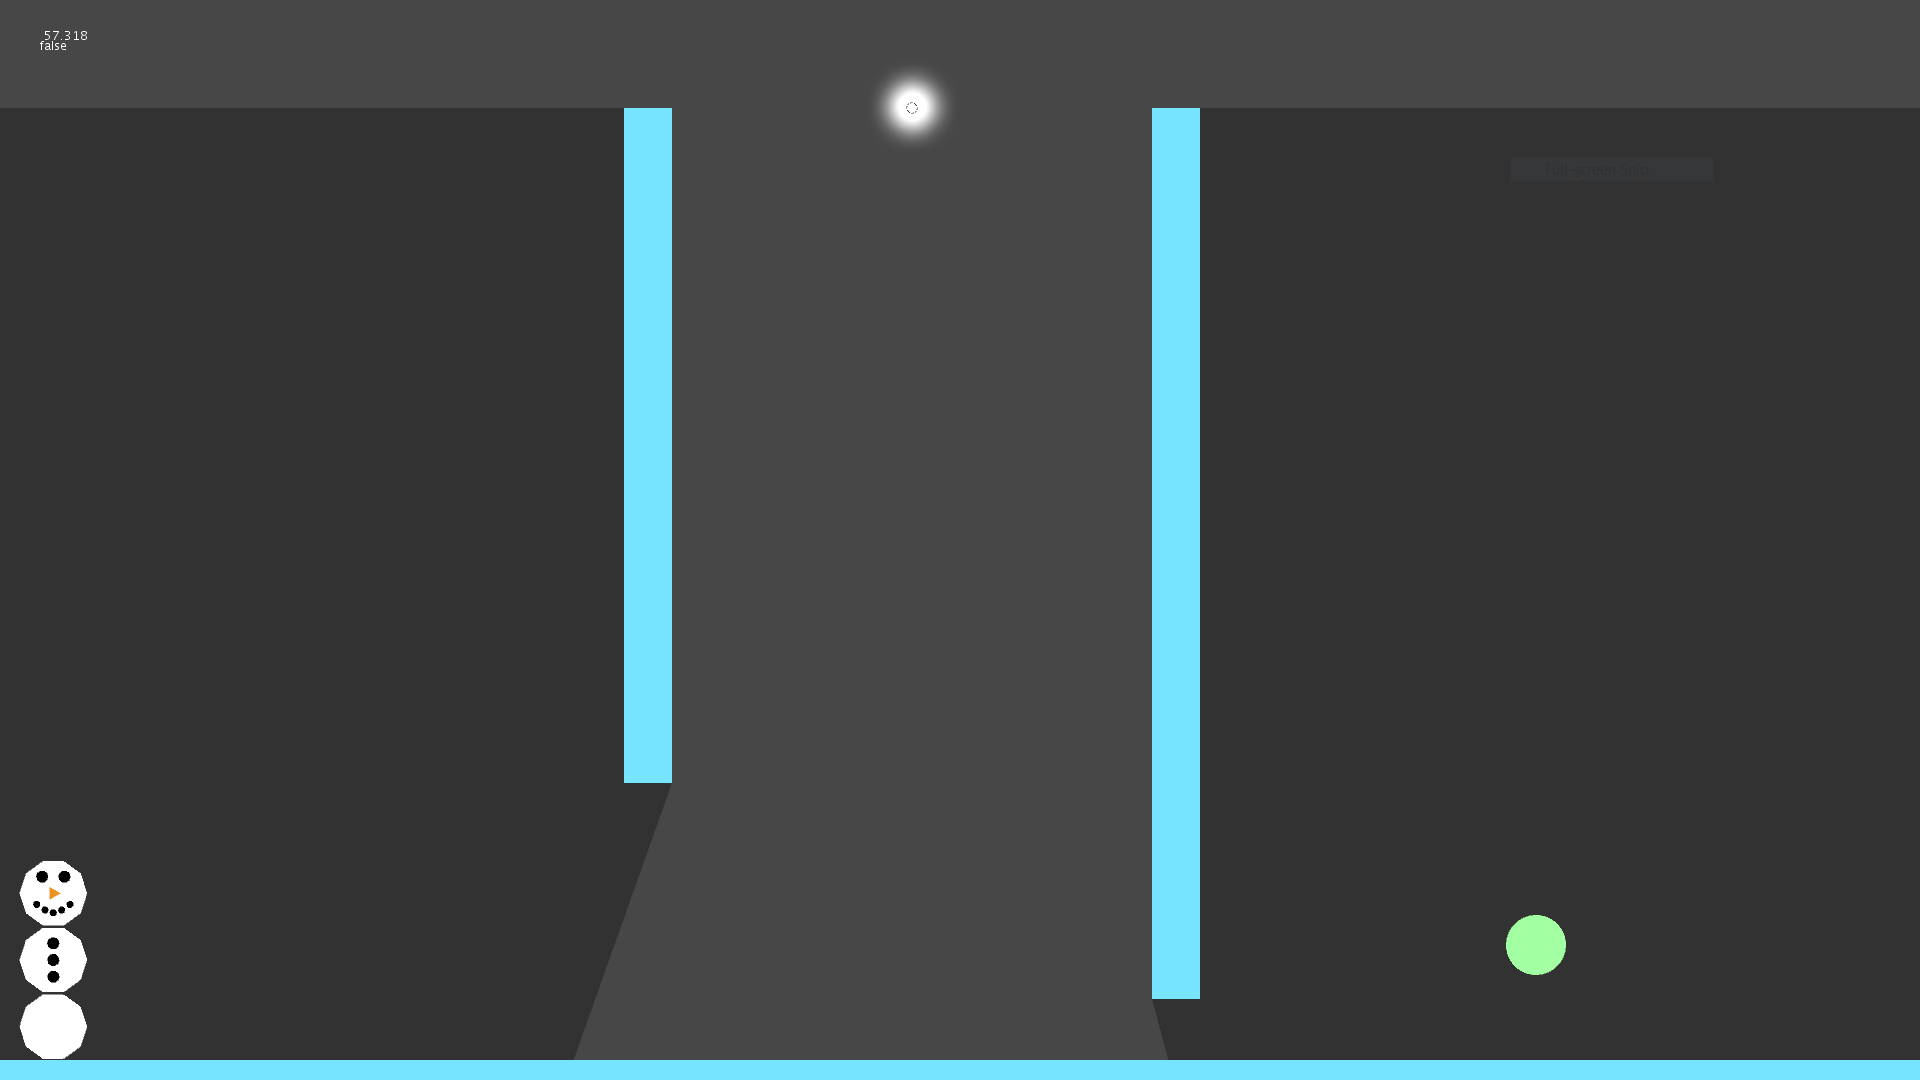
\includegraphics[width=5in]{Frosty.png}
\caption{Starting Position}
\end{figure}

\begin{figure}
\centering
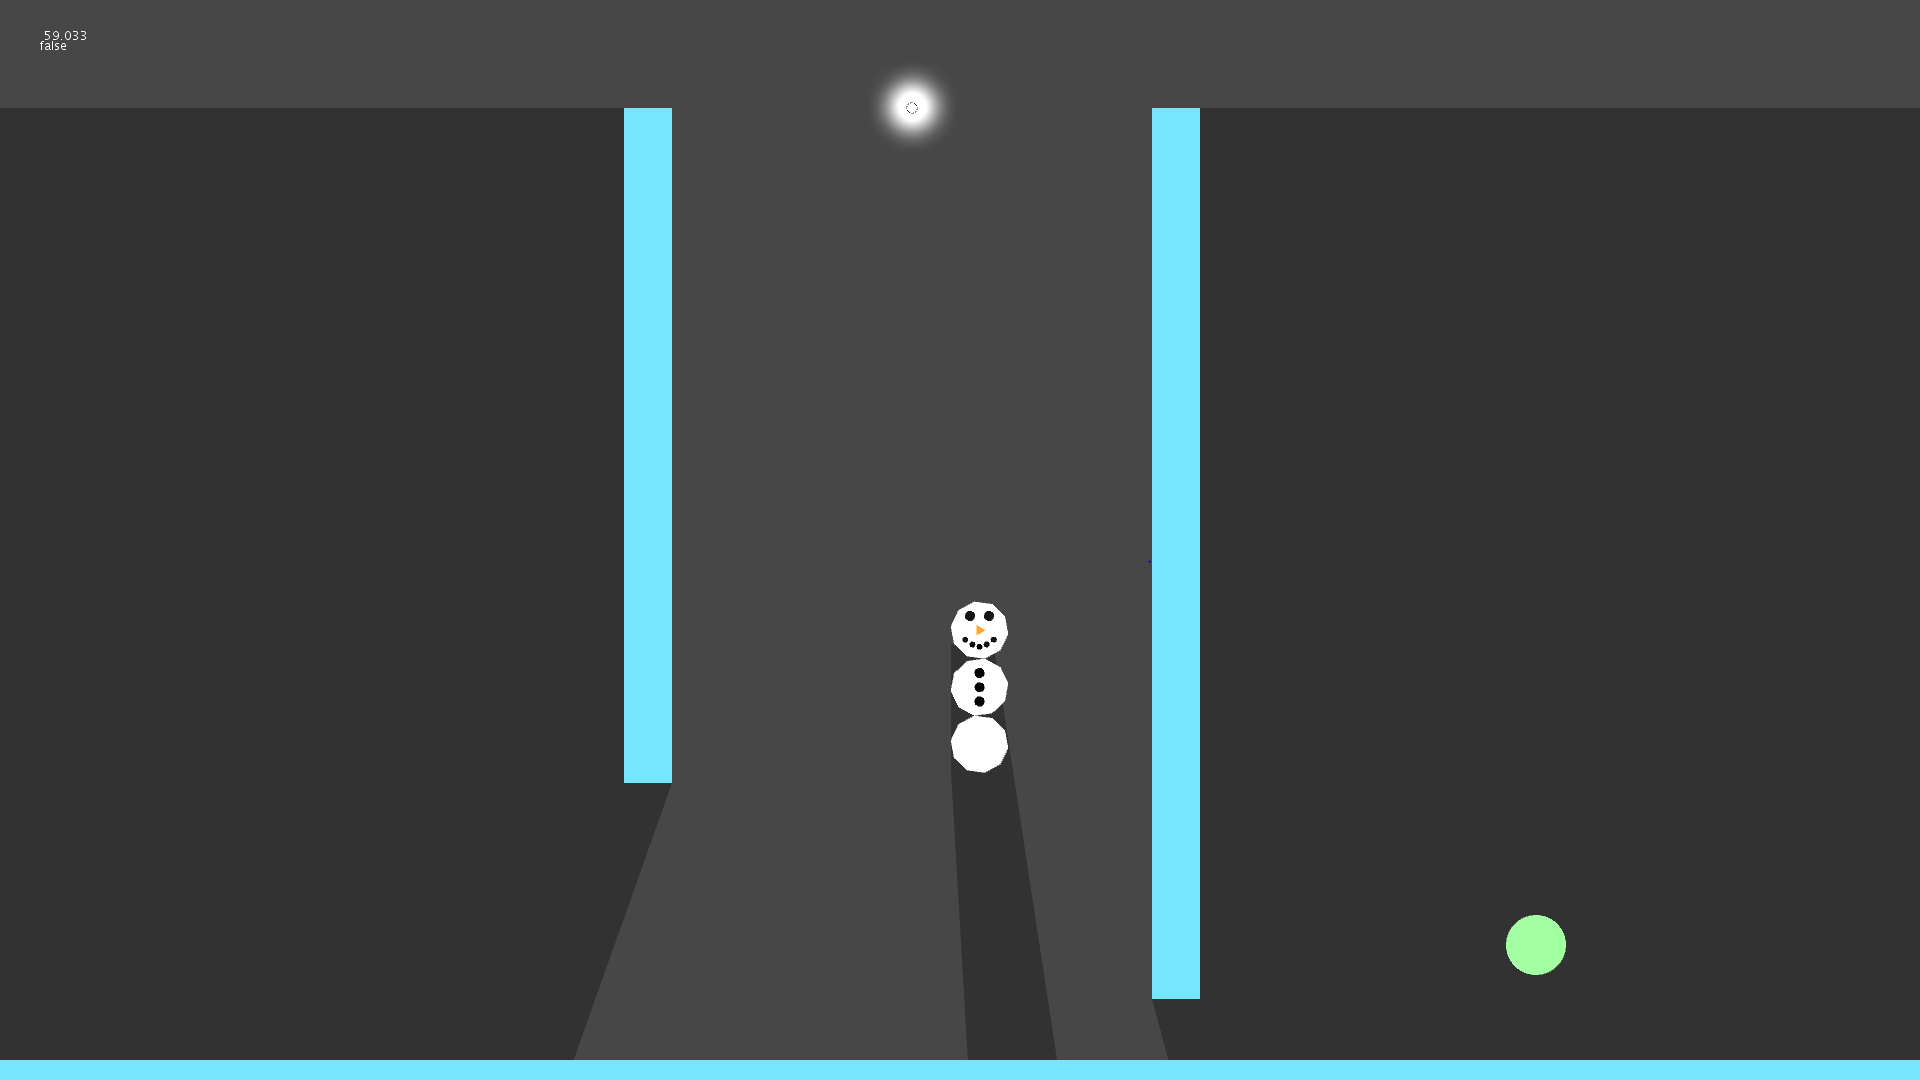
\includegraphics[width=5in]{Shadow.png}
\caption{Jumping to cast a shadow}
\end{figure}

\begin{figure}
\centering
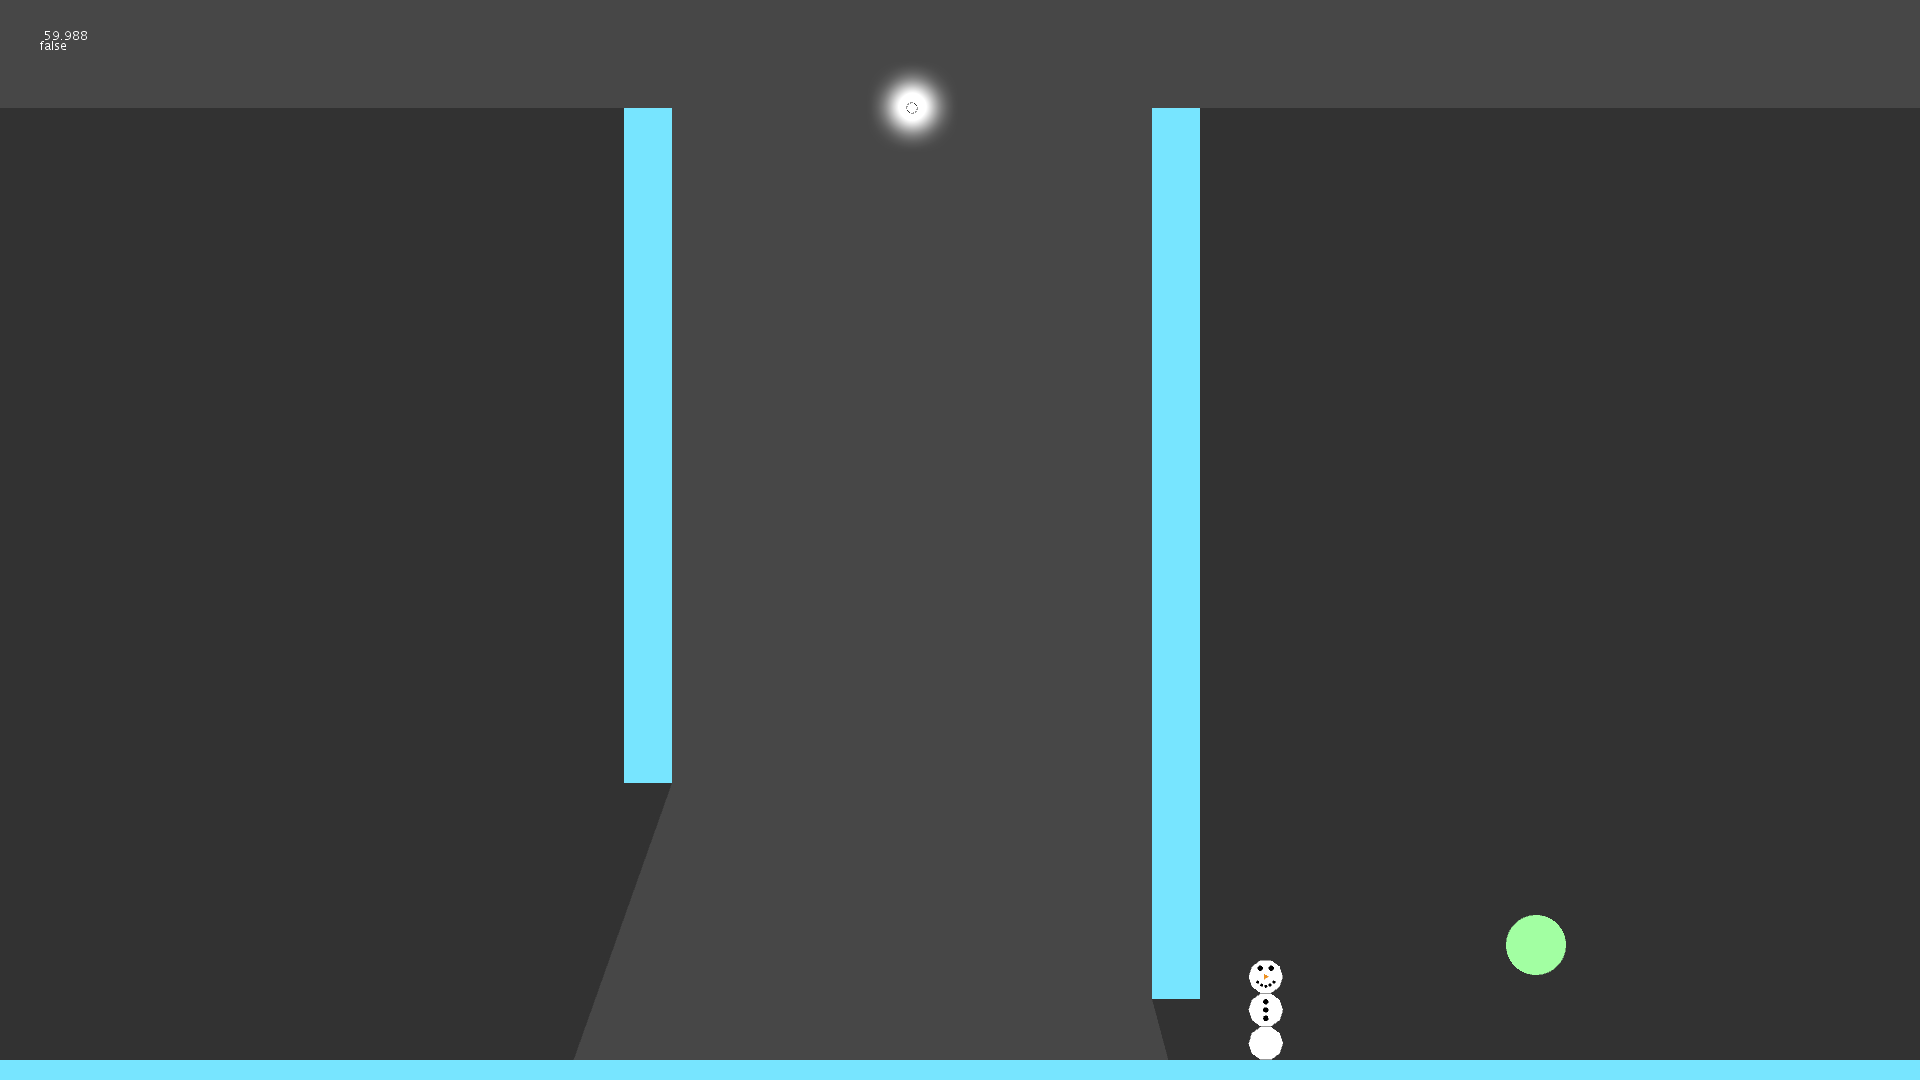
\includegraphics[width=5in]{Shrunk.png}
\caption{Squeezing through after shrinking}
\end{figure}

\section{Discussion}

Overall our results are very encouraging, and are motivating us to improve upon our work.  We are looking into reworking the collision detection system to make it more robust, possibly at the cost of efficiency, refining our level design, and responding to other feedback concerning the visual aesthetic and artwork of our project.
\par From this project, we have learned that it does not take much to make a simple game, and that you can get a lot of mileage out of some simple ideas, if executed properly.

\section{Conclusion}

Stay Frosty is a showcase of our knowledge of lighting and physics simulation and an opportunity to express ourselves visually. As such, we are excited to continue to work on it in the future.
\end{document}
